%----------------------------------------------------------------
%
%  File    :  thesis.tex
%
%  Authors :  Keith Andrews, IICM, TU Graz, Austria
%             Manuel Koschuch, FH Campus Wien, Austria
%			  Sebastian Ukleja, FH Campus Wien, Austria
% 
%  Created :  22 Feb 96
% 
%  Changed :  14 Oct 2020
%
%  For suggestions and remarks write to: sebastian.ukleja@fh-campuswien.ac.at
% 
%----------------------------------------------------------------

% --- Setup for the document ------------------------------------

%Class for a book like style:
\documentclass[11pt,a4paper,oneside]{scrbook}
%For a more paper like style use this class instead:
%\documentclass[11pt,a4paper,oneside]{thesis}

%input encoding for windows in utf-8 needed for Ä,Ö,Ü etc..:
\usepackage[utf8]{inputenc}
%input encoding for linux:
%\usepackage[latin1]{inputenc}
%input encoding for mac:
%\usepackage[applemac]{inputenc}


\usepackage[english]{babel}
% for german use this line instead:
%\usepackage[ngerman]{babel}

%needed for font encoding
\usepackage[T1]{fontenc}

% want Arial? uncomment next two lines...
%\usepackage{uarial}
%\renewcommand{\familydefault}{\sfdefault}

%some formatting packages
\usepackage[bf,sf]{subfigure}
\renewcommand{\subfigtopskip}{0mm}
\renewcommand{\subfigcapmargin}{0mm}

%For better font resolution in pdf files
\usepackage{lmodern}

\usepackage{url}

%\usepackage{latexsym}

\usepackage{geometry} % define pagesize in more detail

%self added packages
\usepackage{underscore}
\usepackage{longtable}
\usepackage{graphicx}
\usepackage{array}
\usepackage{booktabs}
\usepackage{tabularx}
\usepackage{float}



\usepackage{colortbl} % define colored backgrounds for tables

\usepackage{courier} %for listings
\usepackage{listings} % nicer code formatting
\lstset{basicstyle=\ttfamily,breaklines=true}

\usepackage{graphicx}
  \pdfcompresslevel=9
  \pdfpageheight=297mm
  \pdfpagewidth=210mm
  \usepackage[         % hyperref should be last package loaded
    pdftex, 		   % needed for pdf compiling, DO NOT compile with LaTeX
    bookmarks,
    bookmarksnumbered,
    linktocpage,
    pagebackref,
    pdfview={Fit},
    pdfstartview={Fit},
    pdfpagemode=UseOutlines,                 % open bookmarks in Acrobat
  ]{hyperref}
\DeclareGraphicsExtensions{.pdf,.jpg,.png}
\usepackage{bookmark}

\usepackage[title]{appendix}

%paper format
\geometry{a4paper,left=30mm,right=25mm, top=30mm, bottom=30mm}

% --- Settings for header and footer ---------------------------------
\usepackage{scrlayer-scrpage}
\clearscrheadfoot
\pagestyle{scrheadings}
\automark{chapter}

%Left header shows chapter and chapter name, will not display on first chapter page use \ihead*{\leftmark} to show on every page
\ihead{\leftmark} 	
%\ohead*{\rightmark}	%optional right header
\ifoot*{Vincent Oliver Schauer}		%left footer shows student name
\ofoot*{\thepage}		%right footer shows pagination
%---------------------------------------------------------------------

%Start of your document beginning with title page
\begin{document}


% --- Main Title Page ------------------------------------------------
\begin{titlepage}
\frontmatter

\begin{picture}(50,50)
\put(-70,40){\hbox{
\includegraphics{resources_qu/pictures/logo.png}}}
\end{picture}

\vspace*{-5.8cm}

\begin{center}

\vspace{6.2cm}

\hspace*{-1.0cm} {\LARGE \textbf{Declarative vs. Imperative UI Development\\}}
\vspace{0.2cm}
\hspace*{-1.0cm}Differences between the two approaches displayed with a real app\\

\vspace{2.0cm}

\hspace*{-1.0cm} { \textbf{Bachelor Thesis\\}}

\vspace{0.65cm}

\hspace*{-1.0cm} Submitted in partial fulfillment of the requirements for the degree of \\

\vspace{0.65cm}

\hspace*{-1.0cm} \textbf{Bachelor of Science in Engineering\\}

\vspace{0.65cm}

\hspace*{-1.0cm} to the University of Applied Sciences FH Campus Wien \\
\vspace{0.2cm}
\hspace*{-1.0cm} Bachelor Degree Program: Computer Science and Digital Communications \\

\vspace{1.6cm}

\hspace*{-1.0cm} \textbf{Author:} \\
\vspace{0.2cm}
\hspace*{-1.0cm} Vincent Schauer \\

\vspace{0.7cm}

\hspace*{-1.0cm} \textbf{Student identification number:}\\
\vspace{0.2cm}
\hspace*{-1.0cm} c1810475090 \\

\vspace{0.7cm}

\hspace*{-1.0cm} \textbf{Supervisor:} \\
\vspace{0.2cm}
\hspace*{-1.0cm} Leon Freudenthaler, BSc MSc \\

\vspace{0.7cm}

% Reviewer if needed
%\hspace*{-1.0cm} \textbf{Reviewer: (optional)} \\
%\vspace{0.2cm}
%\hspace*{-1.0cm} Title first name surname \\


\vspace{1.0cm}

\hspace*{-1.0cm} \textbf{Date:} \\
\vspace{0.2cm}
\hspace*{-1.0cm} 30.05.2022 \\

\end{center}
\end{titlepage}

\newpage

\vspace*{16cm}
\setcounter{page}{1}

% --- Declaration of authorship ------------------------------------------
\hspace*{-0.7cm} \underline{Declaration of authorship:}\\\\
I declare that this Bachelor Thesis has been written by myself. I have not used any other than the listed sources, nor have I received any unauthorized help.\\\\
I hereby certify that I have not submitted this Bachelor Thesis in any form (to a reviewer for assessment) either in Austria or abroad.\\\\
Furthermore, I assure that the (printed and electronic) copies I have submitted are identical.
\\\\\\
Date: \hspace{6cm} Signature:\\


% --- Deutsche Kurzfassung----------------------------------------------------
\cleardoublepage
\chapter*{Kurzfassung}
Der Smartphone-Sektor ist seit dem Anfang des 21. Jahrhunderts rasant gewachsen. Die Anwendungsbereiche, in denen Smartphones in unserem Leben integriert und angewandt werden, sind breiter gefächert als je zuvor. Sie sind, in vielen Aspekten, ein wichtiger Begleiter unseres Tages geworden. Aufgrund dieses Wachstums und weil unsere Smartphones wahre multifunktionale Geräte geworden sind, steigen auch die Hardware-Anforderungen, welche wir an die Geräte stellen. Sie besitzen nicht mehr lediglich eine Kamera und eine Musik App, sondern die Bandbreite an Applikationen, die zur Verfügung stehen, ist sehr groß. Von simplen Apps, wie einem Timer, bis hin zu Apps, welche eine komplexe UI haben, mit mehreren Fenstern und Animationen spannen
sich die unendlichen Möglichkeiten für den Anwender. Das bedeutet aber gleichzeitig, dass die Anforderungen an die Entwickler der Apps auch steigen. Es werden kürzere Entwicklungszyklen erwartet, in denen ein Produkt von der Idee bis zur Marktreife entwickelt werden soll. Deshalb müssen sich auch ( sollten sich auch) die Werkzeuge ständig verbessern, welche benutzt werden, um Apps zu entwickeln. Der bisherige Status quo der Android App Entwicklung war ein imperativer Ansatz. Er beinhaltet viel „boilerplate“ Code. Das bedeutet, dass jede einzelne Komponente präzise bis ins kleinste Detail vom Entwickler selbst definiert werden muss. Google hat mit dem Framework Jetpack Compose auf eine neue Art der Entwicklung gesetzt. Sie wird als „deklaratives Programmieren“ bezeichnet. Dabei wird den Entwicklern viel Arbeit abgenommen, da sie - abstrakt gesagt - nur noch beschreiben müssen, was sie möchten. Somit ist es möglich Komponenten mit viel weniger Codezeilen zu erstellen. Das Framework regelt den Großteil der Arbeit im Hintergrund. Um einen simplen Button zu erstellen, reichen hier nur wenige Codezeilen dafür aus. Im Vergleich dazu benötigte man früher zwei bis drei Dateien, um zum gleichen Ergebnis zu gelangen. Jetpack Compose verspricht, es Entwicklungszyklen zu verkürzen, App - Ideen schneller umsetzbar zu machen und gleichzeitig eine saubere Code- Architektur zu behalten.

% --- English Abstract ----------------------------------------------------
\cleardoublepage
\chapter*{Abstract}
The smartphone sector has been rapidly growing since the early 2000s. The areas in which smartphones are integrated into our lives have expanded vastly and are now an important part of our lives. Because of this growth, the hardware requirements for our phones have increased vastly due to them becoming truly multi-purpose devices. They do not simply just have a camera and a music application installed, but the application range has grown too. From simple timer apps to apps with multiple screens, complex UI hierarchies, and animations. This means that the requirements for app developers have changed too. Many companies want a faster turnover time from an idea to a fully functioning application. Therefore, there is a need for a new approach to developing applications. While the status quo of Android app development utilizes something called "imperative UI development," Google's Android development team has introduced a declarative framework. This promises the developer a faster development cycle and more modular and maintainable applications. Instead of having to write multiple files to display a button, only a few lines of code are needed. The new framework they introduced is called Jetpack Compose. This declarative framework is a set of libraries written in and for Kotlin applications and promises to ease the development process. It comes with a vast feature set that allows the developer to truly focus on writing modern-looking apps while maintaining a clean code architecture.


% --- Abbrevations ----------------------------------------------------
\chapter*{List of Abbreviations}

\vspace{0.65cm}
\begin{table*}[htbp]
		\begin{tabular}{ll}
 AOT & Ahead Of Time \\
API & Application Programming Interface \\
APK & Android Package (Kit) \\
 ART & Android Runtime \\
 DOM & Document  Object Model \\
 GUI & Graphical User Interface \\
 HAL & Hardware Abstraction layer \\
 IDE & Integrated Development Environment \\
 MVC & Model-View-Controller \\
 SDK & Standard Development Kit \\
 UI & User Interface \\
 VM & Virtual Machine \\
 XML & Extensible Markup Language 			
		
		\end{tabular}
\end{table*}

% --- Key terms ----------------------------------------------------
\newpage
\chapter*{Key Terms}
\vspace{0.65cm}
\begin{itemize}
	\setlength{\itemsep}{0pt}
	\item [] Android Development
	\item [] Declarative UI
	\item [] Imperative UI
	\item[] Jetpack Compose
	\item[] XML





\end{itemize}

% --- Table of contents autogenerated ------------------------------------
\newpage
\tableofcontents
\thispagestyle{empty}

% --- Begin of Thesis ----------------------------------------------------
\mainmatter


\chapter{Introduction}
Mobile devices and their applications are playing an increasingly important role in the daily lives of millions of people around the globe. This means the demand for app developers is also growing. To emphasize this, from October until November 2016, the total market share of mobile devices surpassed that of desktop devices. The gap between the two platforms has been growing ever since. As of February 2022, mobile devices have a 55,98\% market share, whereas desktop devices have a mere 41,59\% \cite{Desktopv59:online}. Because of this, not only has the necessity for developers been growing rapidly, but the technologies used to design and create apps for our daily lives have been improving also. Mobile applications are often used instead of laptops and desktop devices, and therefore, many applications have been ported to mobile platforms. The increase of mobile devices and apps being used is a great driver for the development of the tools being used to make them. \newline

The way mobile applications are developed has changed drastically in recent years. Not only have many frameworks and IDEs been improved and introduced, but the paradigms of how apps are structured and designed have vastly changed also. The classic imperative UI development approach has, for the most part, been superseded by a paradigm called declarative UI development.

Imperative UI development has been the main way of structuring mobile apps for many years. This approach represents a programming style, in which the developer needs to precisely define which UI elements need to go where on the screen. These UI elements are usually separate from the application code and are often defined in XML. In addition to that, the behaviour of the individual elements needs to be added manually as well.

The declarative UI development paradigm aims to make the development process of apps and their behaviour easier and more time-efficient. Instead of having separate files where the UI elements and possibly their behaviour needs to be declared, this is now done in the application code itself. In essence, the developer says what he or she wants instead of defining how to get it \cite{ComposeSummit}.

The goal of this thesis is to draw a comparison between the traditional imperative UI development paradigm and the declarative approach, which has attracted a lot of attention in recent years. The focus of the discussion will be on Android UI development. In order to facilitate the comparison in this thesis, multiple mobile development frameworks will be briefly analyzed and compared regarding certain aspects. The main part of this thesis will be on comparing the XML-based approach to the newly introduced Jetpack Compose way of developing Android applications. Jetpack Compose is a framework that allows the developer to create apps in a declarative way. Furthermore, in order to properly showcase the difference between the two approaches, a fully working Android application was implemented.

\chapter{Imperative vs. Declarative UI programming Approaches}
This chapter explains the basic concepts of declarative and imperative UI. Imperative UI approaches are a more traditional way of tackling UI development. It works on the premise of having to specify what the app should look like, what the functionality is, and how it should be implemented. It usually outsources the UI elements to other files, such as XML. It basically requires the developer to provide a step-by-step guide on what is exactly required.\newline

The declarative paradigm of writing GUIs takes a very different approach. As opposed to specifying all the details of what something should look like, the developer describes what the final state of the desired UI should be. If a scrollable list is desired, for example, the developer simply passes a data list into an object and the framework takes care of creating a basic list in the background. The scrollable list itself, though, is also customizable while using the declarative approach. \newline

This chapter will introduce some frameworks used in imperative and declarative UI development and will illustrate each with a simple example. Before diving into the world of UI frameworks, some historical background is given on the topic of smartphones and how app development has evolved over the past two decades.

\section{History of Smartphone App Development} \label{history}
To be able to understand how far GUI development for smartphones has come, we will first take a look at the first smartphones on the market. Or at least the phones, that were smart for their time and paved the path for the devices we hold in our hands today. For the purpose of this thesis, smartphones are phones which offer the use of applications, which exceed the mere use of a normal telephone. These applications were very different and more limited than applications we take for granted today. \newline

One of the first devices fitting this description was the Nokia 9000 Communicator - or just the Communicator -, which was first shipped in early 1996. The applications ranged from being able to fax and having a digital camera, all the way to web browsing, the possibility to write notes and having a serial terminal integrated. The Communicator ran on GEOS 3.0, which stands for Graphical Environment Object System and is a UI interface for DOS devices. The first phone, which was labelled and sold as a smartphone, was the Ericsson R380, which was launched in late 1999. This was also the first mobile phone, which ran on Symbian OS. Symbian is a mobile OS designed for smartphones. It dominated the smartphone market for most of the early 2000s until about 2010. Companies like Nokia extensively relied on Symbian OS and even bought the company in 2008 \cite{SymbianDocs}.\newline

Apps in Symbian were written in C++ \cite{OeillySymbian}. The pattern most used in Symbian application development is the Model-View-Controller (MVC) pattern, which is still a pretty common pattern used today. Symbian applications consist of at least 4 components: Document, AppUI, AppView and Application - and an engine. When trying to compare these components with an MVC pattern, the Application Engine corresponds to the Model and manages application data. The View of MVC matches to AppView. The Controller of MVC is distributed in several different components: Application, AppUI and Document together perform the functionality of the Controller. To create GUIs, Nokia created a designer tool called Carbide.c++ UI Designer, which visual interface is based on the Eclipse IDE. The phones and the apps that were created at this time were not designed for the mass market, but rather for business use \cite{AlmudenaDiazZayas2010}. \newline

The real game-changer in app development and smartphones was in 2007 with the release of the first iPhone. The stylus, which was used previously, was superseded by the touchscreen, which could be navigated with the touch of a finger. Android, developed by Andy Rubin, released the first Android smartphone in 2008, which was the HTC Dream. Although both companies were pioneers at the time, they had very different approaches, which still affect the development of the apps today. Apple's iOS started as closed source, whereas Android has been open source from the beginning \cite{Pothitos2016}. Android was bought by Google in 2005. In 2007 Google held a press release, which stated some goals they had with Android and finally put it on the map. With the introduction of Android - a single OS, which could run on multiple devices - the development process changed rapidly. Now developers could write application code which, with little extra effort, could run on various devices. The rAPId improvement of the Android OS is also because of its open-source nature due to the Apache license. The Apache license states that the software can be freely used, modified and even made proprietary and sold (if modified) \cite{ApacheLicense}. \newline

All of this also entails, that Android applications could be written on any machine. Apple took a very different approach and has had its software under lock and key from the beginning. This forced developers to make iOS apps from apple devices and made it a necessity to own a MacBook or similar. iOS app developers need to use the iOS Software Development Kit (SDK), which gives them access to all the peripherals on iOS devices. Apple has set certain standards for app development on iOS, which limits developers somewhat in what they are allowed to do. This entails that all apps are screened and validated by apple before releasing them on the App Store. This results in a more limited market place but at the same time, there is always a certain quality and security standard which is met. In addition to this, there is also a financial and - in comparison to Android - a high bureaucratic hurdle that developers have to pay and overcome, to publish apps to the app store. Android apps on the other hand are very simple and cheap to publish, which also results in apps landing on the app store that do not necessarily have high security or design standards. Android allows the installation of apps on smartphones via APKs. APK stands for Android Package (Kit) and represents the format of applications that can be installed on Android phones. This makes it possible to install third-party apps onto the phone. Apple officially does not support this, due to quality restrictions. There are some methods though, which allow the installation of third-party apps. Jailbreaking an iPhone is one of them. Jailbreaking is the process of modifying the iOS, to lift the restrictions put in place by Apple. This makes it possible to install apps without having to pass the strict quality bar of the AppStore. \newline

As of January 2022, Android had a total market share of 69,74\% and iOS of 29,49\%. To put that into perspective, Symbian OS has dropped from 47\% in 2012 to 0,1\% in January 2022. \cite{Krajci2013, MobileOSStatistics}

\section{Imperative UI Development Approaches}

\subsection{Apple's UI Development Tools}
Prior to the newly introduced SwiftUI framework, discussed in section \ref{swift_ui}, developers in the Apple ecosystem had multiple different frameworks to create applications. These frameworks are WatchKit \cite{WatchKitDocu}, AppKit \cite{AppKitDocu} and UIKit \cite{UIKitDocu}. Whereas the first two are pretty self-explanatory, UIKit is used to develop applications for iOS and tvOS. These tools follow the previously explained imperative programming approach for UI development.
\begin{itemize}
\item
AppKit\newline
The AppKit is the framework used to develop user interfaces for macOS apps. It handles all the background processes, such as communicating with the hardware, screen buffers, clearing areas of the screen before UI is drawn, etc.
\item
WatchKit\newline
The framework for creating watchOS apps provides the entire infrastructure needed, including Siri intents, extended runtime sessions and much more. The hardware information of the Apple Watch can also be accessed.
\item
UIKit\newline
Since the previous two frameworks cover macOS and watchOS, UIKit takes care of the rest. So it provides the environment to develop apps for iOS and tvOS. It comes with the infrastructure needed to create interfaces and takes care of the event handling for Multi-Touch input amongst other things. It also provides everything needed to implement features such as animations, documentation and accessing the hardware of the devices.

\end{itemize}


\subsection{XML}
A popular form of UI design is by using XML structures. XML is short for Extensible Markup Language and is a standard for storing data in a hierarchical text-based manner. XML files are simply files which store information in a specific layout. They are used to store and transfer information. Depending on the context, there are various kinds of tags which are used to describe the information being stored. The tags available to describe the content of the XML file are defined by a schema, which needs to be created and integrated into the XML document. The schema can be custom made or a publicly available one can be used. Although XML is used in UI development also, its main use is in simple data storage and data transfer. It is heavily used when two distinct systems - who do not necessarily understand each other otherwise - want to communicate or send objects to one another. It also makes serialization easier. This means to turn the objects of code into a byte stream, so it can be transferred over the wire \cite{xmlStandard}. \newline In UI development these XML files would store UI elements and their properties. It must be stated though, that using XML as a way to define UI elements does not make it inherently imperative. Frameworks, such as .NET WPF \cite{WpfXML}, use a modified version of XML and are declarative. \newline

\subsection{Android development using XML}
An environment where XML is heavily used imperatively is in classic Android UI development. Here XML is utilized for creating the elements that make up the UI. In Android development, there are Views and ViewGroups. Views are visible elements on the screen - defined in XML - whereas ViewGroups are a group of Views or other ViewGroups. An example of a View would be a button or a slider, whereas a ViewGroup would be the button and slider together. ViewGroups are therefore invisible containers that contain multiple Views or ViewGroups. Each View, also known as a widget, is then defined by an opening tag and has a subset of attributes which can be used to imperatively describe the View being created. The following code snippet in listing \ref{listviewXML} shows how a ListView is written in XML in Android. The attributes declared in XML can vary from simple IDs and layout constraints, all the way to onClick listeners and many others. This ListView by itself has no functionality though and only represents a View which can then be integrated into the app in code. Unlike in declarative approaches, this way the developer needs to define exactly what the view should look like and how it should do what it does \cite{AndroidXmlLayouts}.

\begin{lstlisting}[caption={ListView in Android XML}, ,captionpos=b,label=listviewXML]
<ListView
android:id="@+id/list"
android:layout_width="match_parent"
android:layout_height="match_parent"/>

\end{lstlisting}

Chapter \ref{ui_dev_android} will discuss this in more detail. \newline

\section{Declarative Framework examples}
There are many UI frameworks on the market. Most of them are written in different languages but are often designed for multiple platforms. Some frameworks, such as SwiftUI from Apple \cite{SwiftUIDocs} are solely developed to work on one platform - all iOS platforms in this case. Other frameworks, such as Flutter \cite{FlutterDocs} are multi-platform frameworks, where much of the code can be shared between platforms and only platform-specific requirements need to be rewritten.

\subsection{Flutter}
Flutter is an open-source framework by Google which uses the declarative UI approach. It is used to build applications, which are natively compiled, multi-platform and stem from a single codebase. Multi-platform in this case means that it runs on Windows, macOS and Linux on the Desktop side of things and IOS, Android and Fuchsia \cite{FuchsiaDocs} on mobile. Additionally, web applications can be written also. Fuchsia is the next-generation OS from Google \cite{Wu2018}. Flutter uses the open-source programming language Dart \cite{DartDocs}, which is a modern OOP language, also predominantly developed by Google. In contrast to many other frameworks, such as React Native, the team at Flutter utilize their own high-performance rendering engine. The rendering engine used is called Skia \cite{SkiaDocs}. This means they do not rely on the device's OEM widgets or, like other frameworks do, use web views. When compiling for Android, the C/C++ engine is compiled with the Android NDK, whereas for iOS LLVM \cite{LLVMDocs} is used. Both are compiled into ARM libraries. Dart code on the other hand is compiled ahead-of-time (AOT) and is compiled into native code \cite{FlutterFAQ}.\newline
Dart, as mentioned before, is a statically typed programming language developed and maintained by Google. Dart was designed to be the successor of JavaScript \cite{Bailey2021}. Originally the idea was to have Dart run on a VM but Google scrapped that idea and instead focussed on compiling it to JavaScript. There are Dart to JavaScript compilers which can be used in systems where Dart is not an option. To please the masses, the Dart development team decided to make Dart look a lot like Java \cite{Bailey2021}. \newline
Flutter implements a so-called hot reload development cycle. This means developers can expect sub-second reload times on a device or an emulator. Hot reload is a stateful approach and works by injecting updated source code files into the running Dart VM. This makes it possible to inject new classes or methods into existing classes, without losing the state. An example of this would be, when a developer is 3 screens into the app itself and injects new methods, it would still be possible to navigate back to all 3 screens \cite{DartFAQ}.

The listing \ref{listviewFlutter} is an example of how to create a list in Flutter. The result is shown in figure \ref{flutter_scrollable_list}.

\begin{lstlisting}[caption={ListView in Flutter}, ,captionpos=b,label=listviewFlutter]
  @override
  Widget build(BuildContext context) {
    const title = 'Basic List';

    return MaterialApp(
      title: title,
      home: Scaffold(
      
        body: ListView(
          children: const <Widget>[
            ListTile(
              title: Text('A List Item'),
              tileColor: Color(0xFFFFCC00)
            ),
            ListTile(
              title: Text('A Second List Item'),
              tileColor: Color(0xFFFF9501)
            ),
            ListTile(
              title: Text('A Third List Item'),
              tileColor: Color(0xFFFF3B2F)
            ),],),),);}
\end{lstlisting}

\begin{figure}[htbp]
\centerline{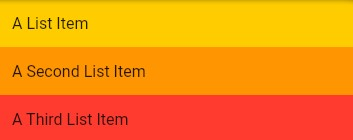
\includegraphics{resources_qu/pictures/flutter_scrollable_list.jpg}}
\caption{ListView in Flutter}
\label{flutter_scrollable_list}
\end{figure}

\subsection{SwiftUI vs. traditional approaches}\label{swift_ui}
As discussed earlier, apps for Apple devices used to be developed with multiple different frameworks, depending on what kind of device was targeted. These frameworks utilize the imperative programming paradigm and come with their own set of issues. One of these is that the way views receive their data is tedious and prone to errors. The reason for this is that all views receive their data via a view controller. This view controller sends data to a view and when changes occur in the view, it then proceeds to write the updated data into models. When references to views change or other unforeseen events happen, this can cause the app to crash. This is a problem which SwiftUI is meant to fix, by introducing state-driven views \cite{Sillmann2020}.

As the name suggests, SwiftUI uses the Swift programming language. Swift is an open-source programming language developed by Apple for developing applications for Apple devices, including iOS, macOS, watchOS and tvOS and uses a declarative syntax \cite{SwiftDocs}. Although there is a project going on where downloadable Swift toolchain images are being made, to use Swift on Windows also. The way it has been done, it is also possible to utilize the Windows system libraries in the Swift programming environment, making for a seamless developer experience \cite{Abdulrasool2020}. Although Swift is a fairly new language, it has many similarities to C and Objective-C., such as structs and other keywords. The Swift language itself is based on C++ \cite{SwiftGithub} but its standard library is written in Swift \cite{SwiftDocs}. In contrast to the older frameworks, AppKit, WatchKit and UIKit, it is not possible to develop UI using Objective-C, instead Swift is mandatory. As mentioned before, SwiftUI introduced state-driven views. This results in the views having direct access to the data they require via data binding. If either the view of the data changes, SwiftUI issues a refresh on the view and the state is updated automatically, without the need of a view controller \cite{Sillmann2020}.

The following code in listing \ref{listviewSwift} shows how to make a list in SwiftUI. Figure \ref{swift_list} shows what the result looks like.
\begin{lstlisting}[caption={ListView in Swift}, ,captionpos=b,label=listviewSwift]
struct ContentView: View {
var body: some View {
List {
Text("A List Item")
.listRowBackground(Color.yellow)
.listRowSeparator(.hidden)
Text("A Second List Item")
.listRowBackground(Color.orange)
.listRowSeparator(.hidden)
Text("A Third List Item")
.listRowBackground(Color.red)
.listRowSeparator(.hidden)
}}}

\end{lstlisting}

\begin{figure}[htbp]
\centerline{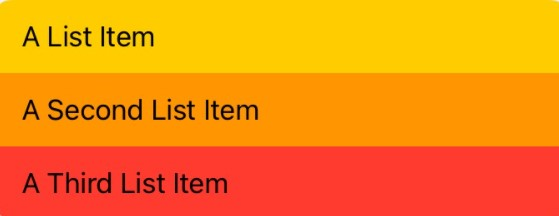
\includegraphics[scale=0.65]{resources_qu/pictures/swiftui_list.jpg}}
\caption{Listview in SwiftUI}
\label{swift_list}
\end{figure}

\subsection{React Native}
React originally was intended to be a simple JavaScript library to create UIs and was founded by Facebook - or now Meta. It was first released in 2013 to aid the development community to create user interfaces. React is nothing more than the view part of the MVC paradigm and is therefore only designed for the client side of development. Although it is also possible to render the UI on the server-side. React follows the declarative approach of programming and can also be viewed as a declarative API wrapped around an imperative one. The way it displays data to a device is by using a virtual DOM, or virtual Document Object Model. The DOM itself is simply a representation in form of a tree structure. It displays the current state of the web page with HTML. Every time the state of the web page changes, for example, the server sends new data, the DOM is either recreated or the contents of the DOM are manipulated by JavaScript \cite{Fedosojev2015}. React utilizes something called a virtual DOM - which essentially selectively renders subtrees of the nodes in the DOM, whenever the state changes. This way only minimal effort is required for the web page to stay up to date. \newline
After a booming success with React, Facebook decided to also dive into the smartphone market. Therefore, at an internal Facebook hackathon, the foundation of React Native was created. Initially, it was meant to be a platform where both Android and iOS apps could be developed. However, as the React Native community and framework grew, they integrated the possibility to deploy applications also to platforms outside the smartphone world, such as the web and Windows. Meanwhile React Native has become a wild success, with not only Facebook and individual contributors adding value to the open-source project, but tech giants such as Microsoft or Samsung as well \cite{Wu2018}. Facebook follows the principle of ''learn once, write everywhere'' which dictates that since it is only the UI that differs on various platforms, it should be written once but then rendered separately on the individual platform required. In contrast to React, which renders all UI elements in the browser, React Native runs in an embedded instance of JavaScriptCore (used for iOS) or V8 \cite{V8Docs} (used for Android) inside the applications. V8 is Google's open-source JavaScript engine. React Native can render components to real native views for either Android or UI views for iOS. This is done by utilizing a concept called ''the bridge''. The bridge is simply an abstraction layer, which makes it possible for React Native to invoke the UI rendering APIs in Java (Android) or Objective-C (iOS). It is also possible to access platform-specific features, such as location services or battery \cite{Danielsson2016}.

As in the previous two frameworks, listing \ref{listviewReact} is also a code example of how to create a list view in the declarative syntax using React Native (the data source is left out for this example). This code then outputs a view shown in figure \ref{react_native_list}.

\begin{lstlisting}[caption={ListView in React Native}, ,captionpos=b,label=listviewReact]
const DATA = [ { title: 'A List Item', },  {title: 'A Second List Item', },{ title: 'A Third List Item',},];

const App = () => {
  const renderItem = ({ item, index }) => (
  index == 0 ? <Text style={[{backgroundColor: '#FFCC00', padding: 20}]}>{item.title}</Text> : 
  index == 1 ? <Text style={[{backgroundColor: '#FF9501', padding: 20}]}>{item.title}</Text> :
  index == 2 ? <Text style={[{backgroundColor: '#FF3B2F', padding: 20}]}>{item.title}</Text> : null  );

  return (
      <FlatList
        data={DATA}
        renderItem={renderItem}
      />
  );
}

\end{lstlisting}

\begin{figure}[!hbt]
\centerline{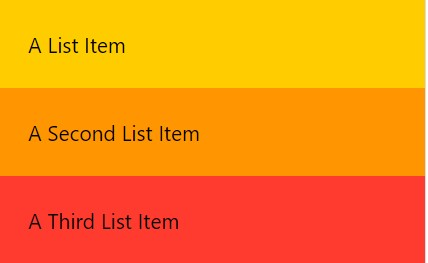
\includegraphics[scale=0.8]{resources_qu/pictures/react_native_list.jpg}}
\caption{Listview in React Native}
\label{react_native_list}
\end{figure}

\subsection{Jetpack Compose}\label{jetpack_compose_introduction}
Jetpack Compose is a Kotlin framework developed by Google for creating native applications using the Kotlin programming language. It was first introduced in the Android Dev Summit in 2019 \cite{ComposeSummit}. The first stable version of the framework was released with version 1.0 in the summer of 2021 \cite{AndroidD83:online}. The framework supports a vast selection of features such as animation previews and component previews. These and the promise of making the app development and design process less tedious are some of the big selling points for Jetpack Compose. This section will cover some basics of Jetpack Compose, whereas chapter \ref{ui_dev_android} will deeply cover the subject and compare Jetpack Compose with the previous way of how android apps were developed. \newline

Jetpack Compose is built on top of the original Jetpack architecture and therefore allows the developer to utilize all the existing and known features as well. It is a framework which enables developers to write clean and modern apps and UIs by incorporating best practices throughout the framework. Instead of XML, which was used previously, the Google team has opted for an approach, where the UI is directly written in Kotlin - the language used to write modern Android applications.\newline
The way UI is created is by using Composables. Simply put, Composables are the units which - as the name suggests - compose the UI. Functions annotated with \lstinline!@Composable! are therefore recognized by Jetpack as a part of the UI. Composables can be all manner of elements like buttons or some data structure, which can then be reused with various data sources to reduce boilerplate code \cite{ComposeSummit}. To properly showcase the Composable functions, the following is a code, listing \ref{listviewCompose} example which results in figure \ref{compose_list}.


\begin{lstlisting}[caption={ListView in Jetpack Compose}, ,captionpos=b,label=listviewCompose]

@Composable
fun MyCustomListView(rowNames: List<String> = listOf("A List Item", "A Second List Item", "A Third List Item")) {
    LazyColumn {
        items(rowNames) { row ->
            Card(modifier = Modifier
                .width(150.dp), shape = RectangleShape, elevation = 4.dp,
            backgroundColor = when(rowNames.indexOf(row)){
                0 -> Color(0xFFFFCC00)
                1 -> Color(0xFFFF9501)
                else -> Color(0xFFFF3B2F)
            }) {
                Text(text = row,
                        textAlign = TextAlign.Start)}}}}
\end{lstlisting}
\begin{figure}[!htbp]
\centerline{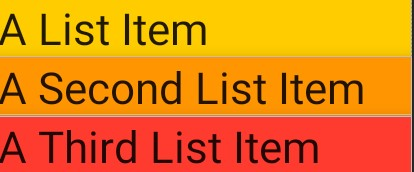
\includegraphics[scale=0.75]{resources_qu/pictures/compose_list.jpg}}
\caption{Listview in Jetpack Compose}
\label{compose_list}
\end{figure}
As is visible in the code example above, the annotation \lstinline!@Composable! is used to make the composables LazyColumn and Card available in this context. \newline

\section{Summary}
This chapter started with a little history of smartphones and app development in general. How smartphones and their applications evolved from - at least from today's standpoint - very basic and primitive technology, to very complex frameworks. These frameworks aid developers to bring all kinds of complex and creative app ideas to life, in a way that the apps are maintainable and preferably scalable. \newline

To sum up this chapter, a summary and comparison of the frameworks will be made here.\newline
Starting with the imperative frameworks, Apple's UI Development kit and XML. Under the hood, Apple's frameworks also use XML files to structure the UI but can manipulate It using a GUI. The same applies to classical Android development.\newline

\chapter{UI development in Android}\label{ui_dev_android}
This chapter starts with a brief recAPItulation of some basic information about Android and its history. It will then go on to explain the architectural stack and finally go on to a deep dive into the comparison of Jetpack Compose and XML UI development in Android. Here the differences between the two approaches will be compared in great detail, ranging from the simple difference in how to create a view, all the way to how animations and other features are implemented. All of this is illustrated with a working Android app, where the features are being implemented. The feature list will not be an exhaustive list of all possible configurations but will give a good insight into how the two ways of creating Android apps differ. To create a context for the features being implemented, the app itself will be explained in section \ref{app explanation}.
\section{Introduction}
As mentioned in chapter \ref{history}, the first smartphone with a fully-fledged Android operating system was released back in 2008. Android was created 5 years prior though and was bought by Google in 2005. The Google Android development team decided to base the Android OS on Linux, an open-source OS. In 2012 Android smartphones surpassed the iPhone in market share and since then Android is the most widespread OS used in mobiles today.

\subsection{Android Architecture}
The Android OS is an open-source project, based on Linux. The Android platform architecture is split into 5 layers. These layers are comprised of system apps, Java API framework, libraries, hardware abstraction layer and finally the Linux kernel. Technically the power management is a layer below the Linux Kernel, but this is neglected in this list \cite{AndroidPlatformArchitecture}.
\begin{enumerate}

\item
Applications\newline
The application layer is where the typical user resides. Apps that are installed are visible here. The Android OS is shipped with various pre-installed apps, such as email, SMS, maps, calendar, contacts and many others depending on the brand of the phone. Many companies which manufacture Android phones ship their own versions of the OS with their own set of apps. Most of the apps installed can be uninstalled, although some can only be deactivated. The apps that are shipped with the phone have no special status. This means, that although a specific browser or email client might be pre-installed, the user is free to install a third-party app and select it as default for browsing or most other kinds of applications. \newline
The apps that come pre-installed not only have a positive impact on normal users but developers might leverage these in their own applications. If a developer wants to include the functionality of the SMS messenger, it would be possible to invoke the messenger from a different app and make it send a message.
\item
Java API Framework\newline
This layer enables the developer to access Android OS features via a set of APIs written in Java. Through these APIs, it is possible to develop Android apps using the core, modular system components and services. Some functionalities, such as location manager can be used in the app development:
\begin{itemize}
\item
Notification Manager\newline
As the name suggests, this manager allows notifications to be displayed in the status bar.
\item
Resource Manager\newline
This manager simply allows the developer access to non-code resources. These include graphics, layout files, etc \cite{AndroidPlatformArchitecture}.
\item
Location Manager Providers
The Location Manager provides the user with the functionality to obtain the device's geographical location. This is an example of an API which requires explicit permission from the user, to function \cite{LocationManager}.
\end{itemize}

\item
Native C/C++ Libraries and Android Runtime (ART)\newline
There are many components of the Android system that are built from native C/C++ code and require native libraries also written in C/C++. Two of these Android system components are the hardware abstraction layer and the Android runtime. Some of these native libraries of the Android system components are accessible via Java APIs which the Android system provides. Although it is also possible to directly communicate with some of these native platform libraries via the Android NDK. \newline
Starting from Android version 5.0 - API level 21 - or above, each app running on a device runs in its own process and with its separate instance of the Android runtime. A couple of features included in the ART are Optimized garbage collection or Ahead of Time (AOT) compiling.

\item
Hardware Abstraction Layer (HAL)\newline
Simply put, HAL allows developers to access hardware functionality from their apps. These can include audio, Bluetooth, camera and many more. These components are accessible via standard interfaces that are exposed to the higher-level Java API framework.


\item
Linux Kernel\newline
The Linux version which Android relies on is the 4.x kernel. It started with the 2.6 kernel but has since undergone 2 major changes. This is where Android gets all its core system functionality from, such as process management, network stack, memory management, security and others. The entire Android platform, such as the Android runtime, relies on the Linux kernel \cite{AndroidPlatformArchitecture}. The Linux version itself is available at \cite{AndroidKernelDownload}.
\end{enumerate}


\chapter{Comparison of Jetpack Compose vs. XML}
This is the main chapter of this thesis. It will, in some detail, cover the differences between the traditional imperative way of programming Android applications, with the newly published Jetpack Compose approach. To make this comparison feasible, a real working Jetpack Compose application was developed for this purpose, so the differences can be compared in a proper context. Although many aspects of the UI development, such as UI widgets, state, the architecture of apps, etc. will be discussed, it will not be an exhaustive comparison, because that would go way beyond the scope of this thesis.

\section{Traditional Android Development using XML}
The XML approach is the way apps were designed before Jetpack Compose. Although it is worth mentioning, that most apps on the market - as of the writing of this thesis at least - are still being developed using XML. This is because Jetpack Compose has only been released in its stable form at the beginning of this year \cite{AndroidD66:online}. Many existing apps (and dare I say new ones also) still use Java, although Android has been Kotlin first since Google I/O in 2019 \cite{GoogleIO2019}.\newline
Every Android App requires a so-called Activity. An activity is a screen of an app. Without an activity, the app would not be able to display any UI elements. All UI elements - also called fragments - are loaded into the activity and made visible by it. Many apps consist of multiple activities, while others use a single activity. This depends heavily on the size, the architecture and use cases of the app. The way Android apps are developed, when using XML, is by writing so-called layout files in XML, which are then loaded into the activity and rendered by it. This chapter will go through the main architecture of how Android apps are built using XML. It will also touch upon some topics, such as navigation and others, to properly portray the comparison between Android development with XML and Jetpack Compose.

\subsection{Layouts}
As mentioned above, activities are responsible for showing UI elements. These elements are defined in so-called layout files. A layout defines the structure of the UI. The layout file itself consists of various XML tags, which in turn represent all the different elements displayed by the activity - such as \lstinline!TextFields!. The UI hierarchy is built on views and view groups, whereas views are UI elements visible to the user and view groups are invisible containers, which contain multiple views. This is illustrated in figure \ref{layout_viewgroups}. As shown, a view group can be part of a different view group and at the same time contain multiple Views. \newline
Before we go on with XML code, views and view groups will be explained a little.

\begin{itemize}
\item Views \newline views, also called widgets, can be a subclass of a variety of different elements. Here are 5 popular views:

\begin{itemize}
\item TextView
\item Button
\item Checkbox
\item Radio Button
\item Date Picker
\end{itemize}
Each View is assigned an ID. This ID is then used to find the view in the view hierarchy generated by the XML files. Values such as the width and height of a view can also be set in XML, but more on that later.


\item ViewGroups \newline
ViewGroups are subclasses of Layout. There are multiple different layout variations, each designed for a different use case. Here are 5 popular layout types:

\begin{itemize}
\item Constraint Layout: This is one of the most popular used layout types. It allows the developer to flexibly position all the views using constraints.
\item Linear Layout: This layout organizes its children into a horizontal or vertical row. A scrollbar is automatically added, in case the row exceeds the display size.
\item Relative Layout: Each child object's location can be specified relative to each other
\item List View: Displays a scrolling single column list
\item Grid View: Displays a scrolling grid of columns and rows \cite{AndroidXmlLayouts}


\end{itemize}
\end{itemize}

\begin{figure}[!ht]
\centerline{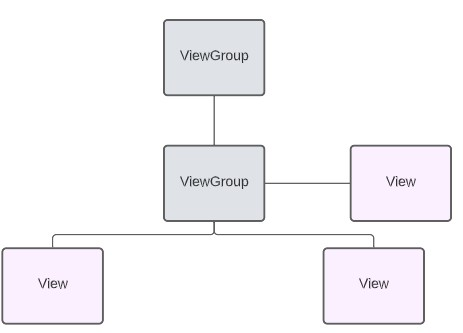
\includegraphics[scale=0.75]{resources_qu/pictures/layout_viewgroups.jpg}}
\caption{ViewGroups hierarchy}
\label{layout_viewgroups}
\end{figure}

\subsection{Activities}
As previously mentioned, activities house all UI elements that compose the Android app. Activities are not just the technology which allows apps to display widgets, but also act as entry points to an application. This is a paradigm, which is a big difference between mobile and desktop applications. Usually, in a desktop application, one opens the application and gets directed to the same screen every time. There are exceptions, but this sequence is the rule. In many mobile applications, on the other hand, it is an expected behaviour to have a specific screen open, depending on from what context the application was launched. If a user clicks on an email address in a social media app, it is expected to not just have the email app open itself, but also to have a new email being composed with the appropriate address. While many applications are comprised of multiple activities, most apps use a MainActivity, which is the standard entry point to an app. Each activity can launch different activities within the same app or start one in a different app. The following will cover the basics regarding activities and the so-called manifest, which is used to configure the attributes of an activity. \newline
The manifest is an XML file, which houses all the activities and their configurations. Here are the three most popular attributes that can be declared here:

\begin{itemize}
\item Declaring activities\newline The only mandatory attribute which needs to be configured in the manifest when creating an activity is the class name of it. See \cite{ActivityAttributeList} for a comprehensive overview of all attributes available.
\item Declaring intent filters\newline This is the configuration which allows an app to be opened from an external input. An example of this is when the user clicks on an address and gets asked by the Android system, which app it should use to open. Every app option being offered has an intent filter built-in for this specific action.
\item Declaring permissions\newline Due to the Android OS sandboxing apps from one another for security reasons, each app must explicitly grant permission to share resources and data. There are multiple types of permissions, each corresponding to a separate use case, like access control to the app or for allowing the app to access the internet.
\end{itemize}

The last important thing to mention about activities is the lifecycle methods. These include:
\begin{itemize}
\item onCreate() \newline In this method, logic should be implemented that should only run once in an activity's lifetime
\item onStart() \newline All the code that maintains the UI should be initiated. When the app reaches this state, it is visible to the user for the first time.
\item onResume() \newline In this state the user can interact with the app. The app stays in this state until the activity is interrupted, for example when the screen is turned off.
\item onPause() \newline Whenever the user leaves the activity, this method is called. This does not mean the activity is destroyed, but simply that it is not in the foreground anymore. It might still be visible though.
\item onStop() \newline As soon as the activity is no longer visible to the user, it enters this state. This might occur when a new activity is launched and covers the entire screen or shortly before \lstinline!onDestroy! is called.

\item onRestart() \newline This state follows \lstinline!onStop()!, as soon as the activity is in the foreground again. It will be followed by \lstinline!onStart()! and \lstinline!onResume()!

\item onDestroy() \newline This state is entered when either the activity gets restarted due to a configuration change or when \lstinline!finish()! is called and the activity gets destroyed.
\end{itemize}
The methods themselves are pretty self-explanatory. It is important to mention, that they get invoked automatically and that they can be overridden to adapt the behaviour when being called. An example of this would be to write \lstinline!onClickListeners! in \lstinline!onCreate()!.

Compared to many other application types, Android apps do not have a typical main method which gets invoked. They instead get launched by invoking specific callback methods that then call certain lifecycle methods.
\cite{ActivitiesDocs}

\subsection{Fragments}
Briefly put, fragments are reusable pieces of UI. If there is a custom piece of UI, like a button or a shape, which occurs multiple times in an app, it is good practise to make that a fragment. This way the fragment can be called multiple times in different locations. Whereas traditional Android development and the new approach with Jetpack Compose both use the paradigm of an activity, fragments are not used in the new library. The basic concept stays the same, but fragments get substituted by Composables, which will be discussed in further detail in section \ref{composables}. Fragments also make the app highly modular. For example, depending on the size of the screen, two columns with a scrollable list are shown or just a single column, if it is a smaller screen. The correct display of the lists is the job of the fragment. If there is a navigation drawer that is optionally displayed, this would be the responsibility of the activity. To be able to maintain the modularity that comes with fragments, it is vital though, that the fragment only contains logic necessary to function, otherwise, unwanted dependabilities arise. As it is the case with activities, fragments are also lifecycle aware and the same methods can be overridden. In addition to that, it is also possible to access an enum class which represents lifecycle states. Both ways are possible to access lifecycle in fragments \cite{FragmentDocs}.

\subsection{Navigation}\label{navigation_xml}
In traditional Android development, the navigation uses the navigation component from the Jetpack library. Including the fact, that there is no XML code needed for UI components, the navigation component is a major difference between traditional Android and development with Jetpack Compose. The navigation itself occurs between the destination fragments of an app. Each activity in an application has a so-called navigation graph or NavGraph for short. The NavGraph is an XML representation of all the destinations a user can navigate to. Although it is saved as an XML file, it is created with a GUI tool called Navigation Editor. Here the individual fragments can be added to the screen and graphically connected if there should be a navigation path between them. Optionally navigation arguments can be included also when navigating from one fragment to the next. Although more often than not, it is good practice to use a shared ViewModel, to share data. A ViewModel is an Android class, which can be inherited from. The main goal of a ViewModel is to separate the UI and the business logic. \newline

Although fragments and ViewModels are both lifecycle aware, they differ greatly. Because of this, another reason why ViewModels are necessary is that fragments do not save data when it is re-loaded. This happens on-screen rotations for example. This means, that if the screen is rotated and the lifecycle method \lstinline!onDestroy()! is called, all the data in the fragment will be lost. ViewModels are also lifecycle aware but live in a different scope. They live in the scope of the activity itself. This means that they survive all lifecycle method calls from fragments, but as soon as \lstinline!onDestroy()! is called from the respective activity, the ViewModel is destroyed also. Therefore the fragment will get a new handle on the ViewModel when the fragment is restarted and retrieve the data to be displayed on the screen \cite{ViewModeDocs}. ViewModels will not be discussed further in this thesis, due to there not being a significant difference between the two approaches regarding their use.\newline

Each NavGraph has a navigation host fragment or NavHost fragment. This fragment has the sole purpose of being the surface that the NavGraph uses to swap all the destinations into. When destinations are added to the NavGraph, the XML file gets extended by all the information necessary. For example, if a path is created between two fragments, the \lstinline!action! attribute is added, with the appropriate attributes. There is also an extra dependency available for the arguments passed, called SafeArgs. This dependency ensures type-safety for the arguments, to mitigate crashes during runtime. It does this by generating classes for all the destinations, requiring the argument type specified \cite{NavigationDocs}.

\subsection{Example Button element in XML}\label{button_xml_example}
The below code in listing \ref{buttonXML} shows a basic button UI element. The id field is necessary to locate the particular view in the view hierarchy. When wanting to bind to the object in code, one needs to invoke a method called \lstinline!findViewById!. This searches in the view hierarchy until it has found the element with said id. This approach is quite tedious and slow, hence the Android team at Google developed a feature called view binding. This feature creates a binding class for each XML layout file, that has been created. The binding class instance in turn holds a reference to each generated class. Because this only needs to be done once and does not need to be tediously repeated, view binding is a lot faster and simpler to use than its predecessor. View binding simply needs to be activated in the \lstinline!build.gradle! file and thereby activated for the entire module. When wanting to have a reference to the UI element in code, one simply needs an instance of the binding object and can access the generated classes. \newline
The rest of the attributes are self-explanatory. The onClick attribute points to a method in code, which is executed when the button is pressed. This, as most attributes, is possible to be set in Java or Kotlin code directly also by getting a reference to the object. \cite{ButtonDocs}.

\begin{lstlisting}[caption={Button in Android XML}, ,captionpos=b,label=buttonXML]

<Button
android:id="@+id/button_send"
android:layout_width="wrap_content"
android:layout_height="wrap_content"
android:text="@string/button_send"
android:onClick="sendMessage" />
\end{lstlisting}


\subsection{Animations}
Animations are a huge topic in Android development and are used often. The use cases range from simple slide-in animations to complex custom animations with rotating flying objects. For this thesis though, only a simple animation will be discussed.\newline
The following listing \ref{animationXML} is an example of what a simple fade-in animation looks like in XML. The alpha value is used to set the opacity of an item. The lower the value, the more transparent it gets. In this example, the alpha value starts off at 0, which is fully invisible. Over the course of one second, the transparency changes to be fully visible.

\begin{lstlisting}[caption={Simple Animation in Android XML}, ,captionpos=b,label=animationXML]
<?xml version="1.0" encoding="utf-8"?>
<set xmlns:android="http://schemas.android.com/apk/res/android"
android:fillAfter="true" >
<alpha
android:duration="1000"
android:fromAlpha="0.0"
android:interpolator="@android:anim/accelerate_interpolator"
android:toAlpha="1.0" />
</set>
\end{lstlisting}

This is an example of a View Animation. There are two types of animation:
\begin{itemize}

\item View Animations\newline
There are Tween and Frame animations. The former performs a series of transformations on a single image and the latter displays a series of images to generate an animation.

\item Property Animations\newline
Property Animation changes the property values of an object. By doing this over a certain amount of time, animations are created.

Animations can be a rather complex topic, but this was a basic overview of them \cite{AnimationXMLDocs}.
\end{itemize}

\section{Jetpack Compose architecture}
Jetpack Compose is a library, which brings multiple modules together into one space. Having a certain understanding of the individual modules enables the developer to write clean apps. It also gives the developer the understanding of when new dependencies are really needed and what levels of abstraction to use, when creating the architecture of the app. The following will briefly illustrate the major layers of Jetpack Compose. Each layer is built on top of the lower layer's public API, which makes it possible to replace any layer if needed.

\begin{enumerate}
\item Material\newline This layer integrates Material Design into Compose UI. This way all the styling, theming, icons, etc. are available.

\item Foundation \newline
The foundation provides all the UI building blocks, for example, row, column or lazy column - which is a scrollable list.

\item UI\newline
The basic UI modules such as tooling, text and graphics are implemented on this layer. Also the features like LayoutNode, custom layouts and modifiers are a result of this layer.

\item Runtime\newline
The bottom layer is responsible for creating the fundamentals of the Compose runtime. This includes things like mutableStateOf, annotations such as @Composable and remember. These are concepts that will be explained in the next section.

\end{enumerate}

The higher one gets in the abstraction layers, the more control is been given up. In other words, to create highly customized apps, it is vital to understand what each layer is responsible for. An example of this would be the animations. If someone would like to animate the colour of a component, this can be done using animateColorAsState API. This only goes so far though. To manipulate the behaviour of the component, so that the colour starts out at a different colour in the first place, one needs to drop down a layer and build upon the Animatable API. See \cite{JetpackComposeArchitecture} for a detailed example of this.


\section{Example Application: Parking Heater Control App}\label{app explanation}
The Jetpack Compose application developed for this thesis is a fully functioning app to control the heating system in parking heaters used in camping vans. The reasoning behind choosing this as a project is that in recent years there has been a huge increase in demand for camping vans \cite{CamperStatistic}. From people buying fully converted vans, to those who convert them themselves. Many vans include a heating system, which either works with diesel or gas. There are other systems, but these are the most common. When travelling with camping vans - especially in winter - the van itself is icy cold inside and it can take up to 20-30 minutes until the heating system starts warming up the van to a comfortable temperature. Many heating systems allow for scheduled run times but in my experience, it is not always foreseeable when one will return to the van. This is the reason why I decided to create an application that allows the user to control their heating system from anywhere, as long as they have an internet connection on their phone and in their van. This way the user could switch on the heating system 30-40 minutes before returning to the van and arrive when it is around room temperature. The purpose of the app is also to have a simple but usable application which illustrates the newly introduced Jetpack Compose framework. \newline

For this thesis, only the Android app was developed. A microcontroller and a REST API, with which the app communicates were not developed out of time constraints. The making of these components is not part of the thesis though. From here onward the app is simply referred to as ''Heater app'' or ''HeaterApp''. As far as UI complexity goes, the Heater app is not particularly complex but includes some features discussed in the following sections. The architecture of the app itself is discussed in section \ref{heater_architecture}.

\section{Heater App Architecture}\label{heater_architecture}
\subsection{System Architecture}
To be able to see the big picture, figure \ref{heater_app_system_architecture} is a representation of the context in which the app will be functioning. The app itself communicates with an LTE router located in the van itself. This is done by utilizing Retrofit \cite{RetrofitDocs} as a REST client on the app side of things and a REST API on the microcontroller. The component referred to as the ''Heating Controller'' is the original controller that ships with the heating system but is limited to local use only. The hypothetical heater being used is this \cite{ChinaStandheizungAmazon}. The hypothetical workflow is as follows:
\begin{enumerate}
\item The user activates the heating system at a specific level from the app
\item This input will then be sent via the REST API to the microcontroller
\item The microcontroller generates a signal and sends this to the heater
\item The heater activates the diesel pump according to the signal and begins to heat the van
\end{enumerate}
Notice that all arrows in figure \ref{heater_app_system_architecture} are bidirectional. This is so that the user in the app gets feedback from the microcontroller if and which signal is being sent and can be displayed in the app itself. The connection between the microcontroller and the heater itself is also bidirectional. This is because the heater gives feedback if there are any errors, such as too little fuel.
\begin{figure}[!ht]
\centerline{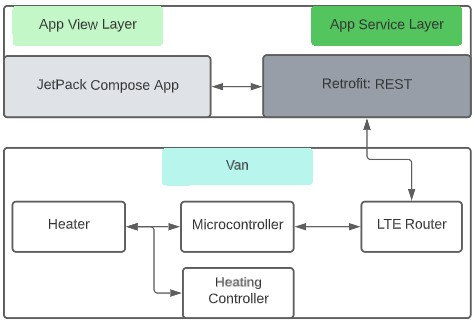
\includegraphics[scale=1]{resources_qu/pictures/heating_setup_architecture.jpg}}
\caption{Heater App System Architecture}
\label{heater_app_system_architecture}
\end{figure}


\subsection{App Architecture}
As visible in figure \ref{heater_app_architecture} the app itself is pretty simple. There are two screens. The HomeScreen is the first screen that appears when opening the app. From there the user can navigate to the SettingScreen to adjust the heater configuration - more on that later. The HomeScreen is the only entry point to the app. What used to be the fragments in the XML approach, are now called screens. The screens communicate with the ViewModel, due to the reasons explained in section \ref{navigation_xml}. The ViewModels then in turn communicate with the repository, which gets its data from the API. The API is the module which sends the REST requests to the microcontroller located in the van, which retrieves its data from a temperature sensor.
\begin{figure}[!ht]
\centerline{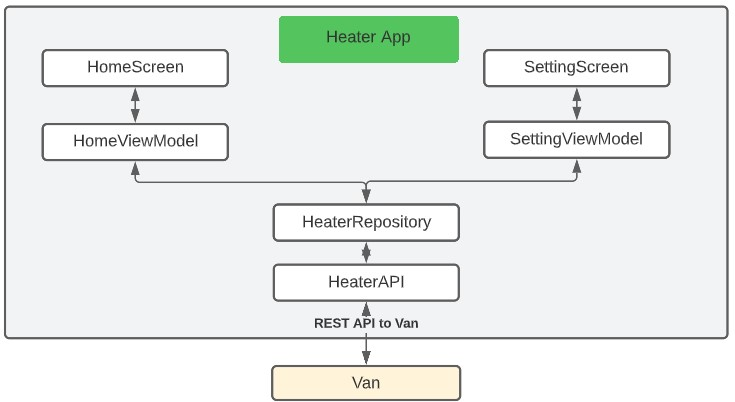
\includegraphics[scale=0.75]{resources_qu/pictures/app_architecture.jpg}}
\caption{Heater App Architecture}
\label{heater_app_architecture}
\end{figure}
\section{Creating Apps with Jetpack Compose}\label{jetpack_compose_gui}
This section will cover the basic workflows, modules and approaches needed to create an app with Jetpack Compose. There will not be any deep dives into any one of the subjects, but a general overview of a fair few of them. When possible, it will be explained with code from the HeaterApp. The emphasis of this section is to showcase the different approaches taken when making apps with the declarative Jetpack Compose library as opposed to the imperative XML approach.

\subsection{Composable functions}\label{composables}
As mentioned in section \ref{jetpack_compose_introduction}, Jetpack Compose, or just Compose, takes an entirely different approach to creating the GUI of an application. Instead of the imperative way of declaring what one would like and how to achieve it, the developer only needs to declare what is desired. Imperative UI development does not necessarily have to entail writing out every aspect of an element oneself. It does however point to a paradigm, which separates the prototype/model of the application's UI and focuses on the what instead of the why. To illustrate a direct comparison between Compose and XML Android development, the following shows how a button is created in Compose. This can be compared to the example XML button shown in section \ref{button_xml_example}.\newline

The code below in listing \ref{composeButton} is a typical way to create a UI element in Compose. The annotation \lstinline!@Composable! changes the behaviour of the function. Functions and or expressions annotated with this can only be called from within another Composable. By annotating a function with \lstinline!@Composable!, implicitly at least, the composable context gets passed into it. This makes it possible to call these composable functions somewhere else, without having to bind to an object first or get the id. It is a standalone callable function. \cite{ComposableDocs}. \newline

\begin{lstlisting}[caption={Button in Jetpack Compose}, ,captionpos=b,label=composeButton]
@Composable
fun BasicButton(name: String) {
Button(onClick = {sendMessage()}) {
Text(text = "Send")
}
}
\end{lstlisting}

As is visible, there is a lot less code required to instantiate and make use of a button in Compose.

Composable functions can also take other composables as an argument, like the composable function with the header of \lstinline!fun MainContent(content: @Composable() () -> Unit)!. This argument can then be called inside the \lstinline!MainContent! function. This feature allows for highly modular and reusable UI code.\newline
A fairly typical paradigm of how the UI code is structured is by creating a package called \lstinline!components! and adding all custom composables here. These composables can then be called from somewhere else in the project and therefore duplicate code is avoided. Any function that emits a UI element, is a composable function. As previously mentioned, composable functions can only be called within a composable function. This means that all UI building blocks, such as buttons, are composables too.\newline

Like in the XML approach, there are layouts in Compose also. Although they are used for the same purpose - to structure the UI elements -, they are simpler to integrate into the UI. What each layout does is pretty self-explanatory. What is often hard though, especially in the beginning, is to know how to arrange and combine them to optimally get the desired result. The standard layouts are:

\begin{itemize}
\item Column\newline
The column layout arranges all elements in a vertical order. It takes 3 main arguments:
\begin{enumerate}
\item Modifier: This will be explained in section \ref{modifier}

\item VerticalArrangement

\item HorizontalAlignment
\end{enumerate}
\item Row \newline
Here the names are similar but subtly different.
\begin{enumerate}
\item Modifier

\item VerticalAlignment

\item HorizontalArrangement
\end{enumerate}

\item Box

\end{itemize}

The reason it is called \lstinline!VerticalArrangement! in the column and \lstinline!VerticalArrangement! in a row, is that arrangement is always respective to the main axis of the layout. Whereas alignment is used to control the spacing of children in the cross axis \cite{ArrangementCompose}.\newline

Although there are other layout types too, such as responsive layouts and slot based layouts. These will not be part of this thesis though.

It is worth mentioning though, that it is not mandatory to use layouts. Composables can be completely free-standing as well. In order to give the elements a structure though, layouts are used \cite{LayoutsComposeDocs}.

\subsection{Modifiers}\label{modifier}

The use of modifiers is a heavily implemented feature in Compose. Every composable takes a modifier as an argument. A modifier is an interface that allows composables to be highly customisable. They augment and modify the composables. They implement the logic necessary to:
\begin{itemize}
\item Change the size, appearance, layout, etc. of a composable

\item Add OnClickListeners

\item Make the composables scrollable, draggable or zoomable

\item etc. The list goes on.
\end{itemize}

When looking through the library code of the modifiers, it is visible that a vast majority of the modifier functionality is based on extension methods. Every extension method in turn returns a new modifier. This makes it possible to chain many modifier methods together. An example of this would be the width modifier in the size library class. The extension method for setting the width of a composable looks like this: \lstinline!fun Modifier.width(width: Dp) = this.then(....){...}!. What the method does is concatenate two modifiers with each other. This means that modifier methods can be chained together, like so:
\begin{lstlisting}[caption={Text in Jetpack Compose}, ,captionpos=b,label=composeText]
Text(
text = "MyTextField",
modifier = Modifier
.clickable { onTextFieldClicked() }
.height(23.dp)
.fillMaxWidth()
)
\end{lstlisting}
This example illustrates not only that multiple methods of a modifier can be chained together but also that any composable can be made clickable. Although Kotlin supports named arguments, it is still best practice for the modifier to be the first argument after the primary argument. The primary argument refers to the argument necessary for the composable to function. \newline

Since each chain makes changes to the modifier, the order of the modifier methods matters greatly. This needs to be taken into account, for example when making an area clickable. If the padding of an element is put before the clickable method, only the non-padded area of the UI element is clickable. \newline

As was visible in the code example above, the height argument takes a dp value as an argument. This does not need to be an Int though, but could also well be a Float, Double, etc. Ultimately though they will all be converted to a Float value. Dp stands for density-independent pixels and is used in all measurements for UI sizes, except for fonts. Fonts use Scalable pixels (sp).\newline

Due to composables often being nested within one another, there are certain modifier functions that only work, when applying them in nested - or child - composables. An example of this would be \lstinline{.matchParentSize()}. For a full list of all modifiers including their scope, \cite{modifierList} is the official documentation for this \cite{ModifierDocs}.

\subsection{State hoisting}
Before getting into state hoisting itself, here is an explanation of what state means in an application. In any application there is data. This data can be anything from a simple variable to a complex database structure. This data can be a constant value or a value that may change over the course of the app's lifetime. State describes all those values that may change while the app is running.\newline

In UI development in general there are a lot of states - as in a lot of data that changes its value over time. This can be as simple as a text field with a counter or a timer that counts down from 100. To keep the app's UI structured, manageable and scalable Jetpack Compose utilizes a paradigm called state hoisting. This simply means that the state is moved to the composable's caller. This way the composable itself is made stateless and is solely responsible for the displaying of the UI. This is done for multiple reasons. One of them is that there is a single source of truth for the data, which gets rid of ambiguity and helps prevent bugs. A second reason would be to make the state shareable between multiple composables that want to access or display the state. This is by no means an exhaustive list of reasons for this design decision.\newline

The general approach for this recommended by Google is to substitute the state variable with two arguments:

\begin{itemize}

\item \lstinline!value :T! which refers to the current value to be displayed

\item \lstinline!onValueChange: (T) -> Unit! which refers to an action that should be taken whenever the value changes, where \lstinline!T! represents the new value.
\end{itemize}

Although this is the proposed method, one is by no means limited to a simple \lstinline!onValueChange! function. This can be replaced by any event deemed appropriate.

A keyword that is often used when talking about state is \lstinline!mutableStateOf!. This creates an \lstinline!MutableState<T>! object which can be observed and is integrated within the compose runtime. \lstinline!MutableState<T>! is an interface which inherits from \lstinline!State<T>! and has a variable \lstinline!value!. Whenever the value changes, it will schedule a recomposition of any composable that accesses it. There are three ways to declare an object of this interface but because they are all equivalent to each other, only one will be illustrated: \lstinline!val myMutableState = remember { mutableStateOf("") }!. This creates an object with the default value of an empty string. Although this is the default way of holding states, Jetpack Compose is not limited to only using this interface. As long as an observable is converted to \lstinline!State<T>! it can be used equivalently. Common observable types that ship with functions to convert them to \lstinline!State<T>! are LiveData, Flow and RxJava2.\newline

Whenever the UI logic involved multiple elements and goes beyond a simple composable call, it is good practice to delegate the state to a so-called state holder. This state holder holds the UI logic and UI elements' state, whereas the composable is solely responsible for emitting the UI elements. Although it is possible to make any class a state holder ViewModels are a good way of going about it. As mentioned in section \ref{navigation_xml} the utilization of ViewModels is a good idea because they outlive configuration changes. ViewModels are also a special state holder class. They are a single source of truth for all UI states and at the same time the layer between different layers, such as databases and API calls and the presentation layer. To make a class a ViewModel, it simply needs to inherit from \lstinline!ViewModel()!. This ViewModel can then be instantiated in a composable in multiple different ways to access the state and logic. This being said, it is possible to have the ViewModel with the logic and a separate class for holding the state \cite{StateCompose}.

\subsection{Animations}
Animations are a big part of many apps. They make transitions between different UI elements feel natural and easy on the eyes. Jetpack Compose comes with a set of animation APIs. Each API is designed for a different purpose. Compose provides many of the APIs as composable functions. These can then be used lust like other UI elements, such as layouts. Google provides a very helpful diagram on their animation documentation site which helps developers choose what API is needed. This can be found at \cite{AnimationComposeDocs}. In general, there are 5 different questions that one needs to ask when deciding which API to pick. Depending on the answer, there are then multiple different options.
\begin{enumerate}
\item Am i animating content change? -> AnimatedVisibility, Crossfade, AnimatedContent
\item Is the animation state-based? -> rememberInfiniteTransition, updateTransition, animateAsState
\item Do I require fine control over animation time? -> TargetBasedAnimation or DecayAnimation
\item Is the animation the only source of truth? -> Animatable
\item Are non of the above applicable? -> AnimationState or animate \cite{AnimationComposeDocs}

\end{enumerate}

To put this into context, listing \ref{heaterSliderAnimationt} is a small example of animation from the heater app. Here the animateColorAsState API is used. It has 2 mandatory arguments:
\begin{enumerate}
\item \lstinline!targetValue! which sets the colour that should be animated towards

\item \lstinline!animationSpec! which defines the type of animation and the duration. In this case, it is a \lstinline!tween! animation, which animates smoothly to the target colour. The opposite to this would be the \lstinline!spring! animationSpec. This jumps abruptly into the next colour. 
\end{enumerate}
In this case, the colour is dependent on the rotation angle of the slider shown in figure \ref{circular_slider}. This gets divided by 360 and rounded. This is done so that the circle is easily dividable into small sections so that the individual temperatures being selected correspond to a warmer or colder colour on the slider. 

\begin{lstlisting}[caption={Heater App Circular Slider Color Animation}, ,captionpos=b,label=heaterSliderAnimationt]
 val circularSliderColor = animateColorAsState(
        targetValue = when ((angle / 360).round(2)) {
            in 0.0..0.15 -> Color.Blue
            in 0.16..0.50 -> Color.Yellow
            in 0.50..0.75 -> CustomColors.Orange
            else -> Color.Red
        },
        animationSpec = tween(
            durationMillis = 500,
            delayMillis = 100,
            easing = LinearOutSlowInEasing
        )
    )

\end{lstlisting}

There are many more animation types, APIs and features that Jetpack Compose has to offer. Listing \ref{heaterSliderAnimationt} just aims to demonstrate how easy it is to integrate animations into an application. 
\subsection{Navigation}\label{navigation}
The navigation aspect of things has changed drastically also. The team at Google has made the navigation very similar to what one would typically use in web development, by employing the paradigm of routes. This will be explained a little later in this section. The basic components, such as NavHost and NavGraph are still the same but have been slightly abstracted and extended. The way it is used - from a developer's standpoint - has changed also. The navigation component is represented by a composable function, which has a reference to the NavHost. This is also a composable function. The destinations themselves are then added by invoking a function called \lstinline!composable!. This function is an extension function of the NavGraphBuilder. By invoking it, the destination - with all its arguments - gets added to the NavGraph. Compared to the previous way of writing Android apps though, there is no graphical way of creating a NavGraph. This makes sense, because there are no individual fragments like before, but instead (many) composable functions in different files, which represent the different screens. \newline

To put all this theory in to practise, listing \ref{heaterNavHost} is the NavHost from the HeaterApp with two destinations, \lstinline!HomeScreen! and \lstinline!SettingScreen! Both do not take any arguments though. If they were to take arguments, the argument name would be appended in the \lstinline!composable! constructor, such as \lstinline!composable(Screens.HomeScreen.name/{name})!. In the use case of the HeaterApp though, it is not necessary. This is also the comparison to web development that was mentioned at the beginning of this section. In web development it is very common to write routes, as if they were URLs.

\begin{lstlisting}[caption={Heater App NavHost}, ,captionpos=b,label=heaterNavHost]
NavHost(
navController = navController,
startDestination = Screens.HomeScreen.name
) {
composable(Screens.HomeScreen.name) {
HomeScreen(navController)
}}

\end{lstlisting}

The screen names on the other hand come from an enum class \lstinline!Screens!. This class looks like the following. First two enums are created and a companion object which has \lstinline!Screens! as a return type. The \lstinline!substringBefore! method is called on the route, to only get the destination name, without the arguments passed.

\begin{lstlisting}[caption={Heater App NavHost}, ,captionpos=b,label=heaterAppScreens]

enum class Screens {
HomeScreen, SettingScreen;

companion object {
fun fromRoute(route :String?): Screens
= when (route?.substringBefore("/")){
HomeScreen.name -> HomeScreen
SettingScreen.name -> SettingScreen
null -> HomeScreen
else -> throw IllegalArgumentException("Route $route is not recognized")
}}}

\end{lstlisting}

When wanting to navigate to a destination, for example by clicking a settings icon, the code for the navigation itself looks like this: \lstinline!navController.navigate(route = Screens.SettingScreen.name)!. The reference to the NavController needs to be retrieved beforehand. This navigation event can be embedded in an \lstinline!onClick! event of an UI element \cite{NavigationDocsCompose}.

\subsection{Canvas}
One pain of the old approach of writing Android apps, that Compose aims to rectify, is the drawing of custom UIs on the screen. This can range from a custom box on the screen in a specific place to a highly complex arrangement of various UI elements in many different styles. An example of this would be a custom logo, like the Instagram logo. Since Compose, the graphic configuration is taken care by Canvas and Compose handles the creating and updating the objects if needed. Having all of this done in a central place has many benefits, like minimizing the amount of state in graphics and having all the options available in one place - in the composable.

The Canvas, as the name already suggests, is a place where the developer can freely draw any graphical objects desired. As it is with all composables, the Canvas is also placed in the layout. Under the hood, Compose takes care of many aspects like state and creating helper objects, etc. This makes the basic use of Canvas quite simple, which does not mean that Canvas can not be used in a little more complex manner, as will be illustrated a little later in this section. \newline

When creating a Canvas, it automatically generates a DrawScope. This is an environment which maintains its own state and also has references to fields that take the parent context into account, such as the size available for the Canvas. The DrawScope also provides the developer with the possibility of drawing any shapes in any location on the screen. Not only different kinds of shapes are supported but manipulations of them also, such as rotations and translations \cite{CanvasDocs}. \newline

In the Heater App this is used to draw a custom circular slider in the middle of the screen. This slider is then used to set either the desired temperature of the van or the frequency, depending what is configured in the \lstinline!SettingScreen! mentioned in section \ref{navigation}.

The circular slider is shown in figure \ref{circular_slider}

\begin{figure}[!htbp]
\centerline{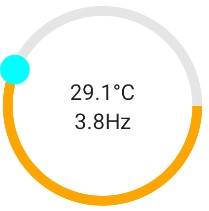
\includegraphics[scale=0.55]{resources_qu/pictures/circular_slider.jpg}}
\caption{Circular Slider to set temperature and the frequency of the heater}
\label{circular_slider}
\end{figure}

This is an example of the use of Canvas, which is not completely trivial and requires some maths also. This is why it will be explained in individual parts. \newline

The first piece of the puzzle, listing \ref{heaterAppCanvas} is instantiating the Canvas object with making heavy use of the modifier argument. Firstly the entire available screen is used for the Canvas. This is done by having references to the other composables relative to the Canvas through the DrawScope. The next argument \lstinline!.pointerInput(Unit)! detects when the circular shape is dragged along the circular slider. It then appropriately sets multiple values needed to display the ball correctly. Finally, a padding is added around the Canvas object, so that there is at least 30.dp space between it and any other composable.

\begin{lstlisting}[caption={Heater App Canvas example: Instantiation}, ,captionpos=b,label=heaterAppCanvas]


Canvas(
modifier = Modifier
.fillMaxSize()
.pointerInput(Unit) {
detectDragGestures { change, dragAmount ->
handleCenter += dragAmount

angle = getRotationAngle(handleCenter, shapeCenter)
change.consumeAllChanges()
}
}
.padding(30.dp)

)
\end{lstlisting}

This part simply draws the gray circle with the defined properties.
\begin{lstlisting}[caption={Heater App Canvas example: drawCircle method}, ,captionpos=b,label=heaterAppDrawCircle]
drawCircle(
color = Color.Black.copy(alpha = 0.10f),
style = Stroke(20f),
radius = radius
)
\end{lstlisting}

This part of the code handles the mathematics behind the dragging event of the slider. It positions the ball correctly, according to the amount it was dragged.

\begin{lstlisting}[caption={Heater App Canvas example: Mathematics}, ,captionpos=b,label=heaterAppMaths]
{
shapeCenter = center

radius = size.minDimension / 2

val x = (shapeCenter.x + cos(Math.toRadians(angle)) * radius).toFloat()
val y = (shapeCenter.y + sin(Math.toRadians(angle)) * radius).toFloat()

handleCenter = Offset(x, y)
\end{lstlisting}
Last but not least, the previous calculations are then used to draw an arc along the grey circle. This arc changes colour, depending on how far along the circle it is drawn. In essence, how high the temperature or the frequency of the heater is set. The hotter the heater gets, the closer to red the arc gets. The \lstinline!drawCircle! is simply the ball which gets dragged along. It takes the \lstinline!handleCenter! as an argument, which was calculated in the previous part.
\begin{lstlisting}[caption={Heater App Canvas example: Draw Arc}, ,captionpos=b,label=heaterAppDrawArc]
drawArc(
color = getColorByAngleValue(angle),
startAngle = 0f,
sweepAngle = angle.toFloat(),
useCenter = false,
style = Stroke(20f)
)
drawCircle(color = Color.Cyan, center = handleCenter, radius = 30f)
}
\end{lstlisting}

This was an example that it is possible to achieve fairly complex things in Canvas, without too much coding, although some understanding of maths is required in this case.

\section{Interoperability between traditional Android development and Jetpack Compose}\label{interop}
Due to Jetpack Compose being a rather new technology, it is not feasible for all apps to be re-written overnight, or at all. Google's Android development team is fully aware of this and has therefore introduced the so-called interoperability APIs. This makes it possible to extend existing View-based android applications with Jetpack Compose composables and vice versa. For this purpose two APIs were developed, Compose in Views and Fragments in Compose.

\begin{itemize}
\item Compose in Views\newline
The ComposeView API makes it possible to seamlessly integrate composable functions into an otherwise XML based android application. For this, it is only necessary to include the correct dependency and call whatever composable desired in the \lstinline!setContent! method.

\item Fragments in Compose \newline
On the other side, there is the AndroidView composable. This makes it possible to integrate Android views into a compose application. This is particularly helpful, when pre-existing complex custom views have been created or when wanting to access UI elements, that are not available (yet) in Jetpack Compose \cite{InteropComposeXML}.
\end{itemize}
\section{Summary}
This chapter gave a somewhat introductory comparison between the view based Android development paradigm and the declarative Jetpack Compose approach. It started with the fundamentals of traditional Android development, to be able to draw a comparison between it and Jetpack Compose. It explained what layouts and activities are and the concepts behind implementing a navigation system with multiple fragments. Finally, before diving into Jetpack Compose, a small example was shown where a button and animation were illustrated. \newline

The chapter then continued by giving a brief overview of the Jetpack Compose framework. For this purpose, a heater application was developed and used to showcase some functionalities of Jetpack Compose. It also illustrated, with some examples, what a Jetpack Compose app looks like and how easy it is to create simple apps with the new framework. By no means was this all that Jetpack Compose has to offer but it serves as a brief introduction.\newline

\chapter{Conclusion}
This thesis aimed to draw a broad comparison between traditional android development and the newly introduced framework Jetpack Compose. The comparison was not solely designed to showcase differences between modern and traditional approaches but was meant as a means to compare declarative and imperative UI development. The thesis started by creating a context for the modern-day smartphone market with a brief historic overview of the various phones that were introduced in the early 2000s. The first smartphone, that could be labelled as such, was Apple's iPhone with a closed source approach. Soon after Android was introduced and has been open source since the beginning. Over the years the Android market share exceeded Apple's and has dominated the market ever since. \newline
After having established a historic context, a brief overview of multiple different imperative and declarative frameworks was given. For each framework, a small example code was given to illustrate what a listview would look like. With this overview, it was visible that the tendency for modern UI development approaches is going towards declarative approaches. Apple used to use AppKit and other imperative frameworks to develop their products and then moved to the declarative SwiftUI approach. The same goes for Android with the old XML based system and nowadays opting for the declarative Jetpack Compose system.\newline
The main part of this thesis was the comparison between Jetpack Compose and the view-based Android approach to developing mobile applications. For this purpose, a small heater application was developed. First, the traditional Android app development system was superficially introduced. All major components to develop a simple app were touched upon and explained with some examples. This part was then concluded with an example of a button and a simple animation in XML. \newline After having established the status quo, the general architecture of Jetpack Compose was outlined. In order to have a context in which to illustrate Jetpack Compose, the heater app was introduced. For this, there were multiple different figures displaying the architecture and purpose of the app. This app was then used to illustrate some example features in Jetpack Compose in section \ref{jetpack_compose_gui}. This section started by explaining the basics of the declarative framework, such as composables - the modular UI blocks, which make up the UI. Furthermore, different concepts such as modifiers and state hoisting were explained in modest detail. The section went on by explaining how navigation and animations were on a basic level with an example. Finally, canvas, the library which allows the developer to draw anything on the screen, was introduced. This was illustrated with an example of a circular slider from the heater app. Before summing up the chapter and concluding the thesis, section \ref{interop} introduced an interoperability API. This API can be used to integrate XML based Android development into Compose and the other way around.\newline

Summed up, Jetpack Compose has successfully managed to ease the UI development of Android applications. By writing all UI elements in Kotlin, it is easy to write a modular UI, which is easily extendible. Because of the declarative approach of simply having to call a button composable for example, it is fast to write a simple UI in a matter of minutes.


\chapter{Future work}
Because of the small scope of this paper, many things could not be addressed or implemented. Nevertheless, here are some potential ideas for further research on this topic:

\begin{enumerate}
\item Implementing the microcontroller part of the heater app\newline
This first point has nothing to do with Jetpack Compose but with the app developed for this thesis. Because of some complications, it was not possible to implement the microcontroller part of the heater app. This was due to measurement issues from the existing heating controller. Due to the heater and the controller having a feedback system, I could not differentiate between the signals being sent.

\item Maintenance comparisons between Jetpack Compose and XML based Android\newline
It would be interesting to research how much effort it is to maintain an app written with both approaches. I would assume that, at least until Jetpack Compose is more stable, the declarative app would need more frequent maintenance. In this regard, it would interest me also, how easy it is to extend each app after several years of not having looked at the project. By this, I mean, which of the two apps would be faster to understand and to add new features to.

\item Performance Comparisons\newline
A further area of research would be how resource demanding XML apps are in comparison to Jetpack Compose apps for the smartphone.

\item Creating a minimum viable product \newline
Because compose is a more compact and intuitive approach, it would be interesting to see how long it would take to make an MVP with XML and Jetpack Compose.

\item Automatic Porting Tool\newline
An interesting area would be to research if it were possible to automatically parse XML UI elements into composables. It probably will never be possible to convert entire apps with a single click, but perhaps parts of the UI.
\end{enumerate}


\newpage

% --- Bibliography ------------------------------------------------------

%IEEE Citation [1]
\bibliographystyle{IEEEtran}
%for alphanumeric citation eg.: [ABC19]
%\bibliographystyle{alpha}

% List references I definitely want in the bibliography,
% regardless of whether or not I cite them in the thesis.

\newpage
\addcontentsline{toc}{chapter}{Bibliography}
\bibliography{literatur}

\newpage

% --- List of Figures ----------------------------------------------------

\addcontentsline{toc}{chapter}{List of Figures}
\listoffigures


% --- List of Tables -----------------------------------------------------

\newpage
\addcontentsline{toc}{chapter}{List of Tables}
\listoftables



\end{document}
